\documentclass[11pt]{article}

\usepackage[utf8]{inputenc}
\usepackage[T1]{fontenc}
\usepackage{lmodern}
\usepackage{graphicx}
\usepackage[left=2cm,top=0cm,right=2cm,bottom=2cm]{geometry}

\pagenumbering{gobble}

\title{\textbf{Förderantrag}}
\author{Zum Aufbau eines LoRaWAN Gateways}
\date{}

\begin{document}

\maketitle

Bei LoRaWAN (kurz für "Long Range Wide Area Network") handelt es sich um einen auf Energieeffizienz und Reichweite optimierten Funkstandard im nicht lizensierten 868MHz Band. Das bedeutet also, dass jeder ohne Funklizenzen besitzen zu müssen ein LoRaWAN Endgerät in Betrieb nehmen kann. Solche Geräte senden dann Nachrichten an einen LoRaWAN Gateway welcher diese dann an einen zugehörigen Server weiterleitet.
Der Aufbau eines solchen Zugangspunktes zum Internet via LoRaWAN steht also voll im Bürgernetzgedanken technische Infrastruktur für jedermann Nutzbar zu machen.

Zur Verknüpfung mit dem Internet hat sich im privaten Bereich vor allem "The Things Network" durchgesetzt, welches eine Infrastruktur zur Verfügung stellt um Nachrichten von LoRa Endgeräten an ihre zugehörigen Dienste im Internet weiterzuleiten. Wie in dem Bild unten zu sehen ist gibt es rund um Pfaffenhofen bereits einige Zugangspunkte: In Ingolstadt, Aichach und Freising. In Pfaffenhofen selbst gibt es jedoch noch keinen.

\begin{figure}[h]
	\begin{center}
		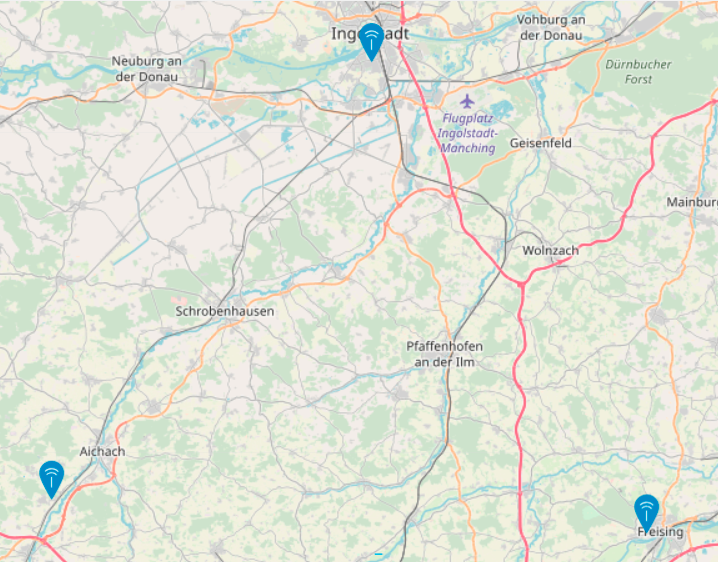
\includegraphics[width=0.5\textwidth]{ttn_paf}
	\end{center}
	\label{fig:ttnmap}
	\caption{The Things Network Abdeckung}
\end{figure}

Zur optimalen Reichweite empfiehlt es sich den Gateway möglichst hoch und mit freier Sicht in alle Richtungen aufzuhängen. In Pfaffenhofen gibt es ein Bunkergelände mit 447m über NN. Dort sind auch die nötigen Anschlussmöglichkeiten (Strom und Internet) gegeben. Der Ortsverband des Deutschen Amateur-Radio-Club e.V.s, der dort auch untergebracht ist, hat zwar selbst kein Interesse an dem Betreiben eines solchen Gateways, hat uns aber Angeboten seinen Antennenmasten mitzubenutzen.

Konkret bitten wir um eine Förderung  mit 70\% der folgenden Anschaffungen:
\\
\begin{figure}[h]
	\begin{center}
		\begin{tabular}{l l}
			\textbf{Beschreibung} & \textbf{Betrag (EUR)} \\
			\hline
			Lorank 8 (LoRaWAN Gateway) & 543.99 \\
			20m CAT.7 Kabel & 15 \\
			PoE Adapter & 10 \\
			\hline
			\textbf{Summe} & 568.99 \\
		\end{tabular}
	\end{center}
	\label{fig:costs}
	\caption{Kosten}
\end{figure}

\end{document}
